% TODO:

% Write ``Liquid-vapor interface'' section A.

% Look up question-mark references (citations).

\documentclass[letterpaper,twocolumn,amsmath,amssymb,prb]{revtex4-1}
\usepackage{graphicx}% Include figure files
\usepackage{dcolumn}% Align table columns on decimal point
\usepackage{bm}% bold math
\usepackage{color}

\newcommand{\red}[1]{{\bf \color{red} #1}}
\newcommand{\blue}[1]{{\bf \color{blue} #1}}
\newcommand{\green}[1]{{\bf \color{green} #1}}
\newcommand{\rr}{\textbf{r}}
\newcommand{\xx}{\textbf{x}}
\newcommand{\refnote}{\red{[ref]}}

\newcommand{\fixme}[1]{\red{[#1]}}

\newcommand{\derivation}[1]{#1} % Use this to show all derivations in detail
%\newcommand{\derivation}[1]{} % Use this for nice pegagogical paper...

% needsworklater is used to annotate bits that need work, but that we
% can postpone for a while.
\newcommand{\needsworklater}[1]{\emph{[#1]}}
% needsworknow is intended to prioritize stuff that needs fixing.
\newcommand{\needsworknow}[1]{\textcolor{red}{[\emph{#1}]}}

\begin{document}
\title{A Fundamental Measure Theory Functional for Hard-Sphere Contact Densities}

\affiliation{Department of Physics, Oregon State University, Corvallis, OR 97331}
\author{Jeff Schulte}
\author{Chris Haglund}
\author{Patrick Kreitzburg}
\author{David Roundy}


%%%%%%%%%%%%%%%%%%%%%%%%%%%%%%%%%%%%%%%%%%%%%%%%%%%%%%%%%%%%
\begin{abstract}
  We investigate the contact density of an inhomogeneous hard-sphere
  fluid, which is of particular interest, as it plays a critical role
  in Statistical Associating Fluid Theory (SAFT), which is the basis
  of a number of recent classical density functionals.  We derive a
  formula for the contact density from the White Bear version of the
  Fundamental Measure Theory functional~\cite{roth2002whitebear}, and
  test this functional agains Monte Carlo simulations.
  \textcolor{red}{Insert summary of results here...}
\end{abstract}

\maketitle

%%%%%%%%%%%%%%%%%%%%%%%%%%%%%%%%%%%%%%%%%%%%%%%%%%%%%%%%%%%%
\section{Introduction}

% The following are papers that use a SAFT-based classical DFT with at
% least some of the terms purely local
\newcommand\saftlocaldft{felipe2001examination, gloor2002saft,%
  gloor2004accurate, clark2006developing, gloor2007prediction,%
  kahl2008modified, gross2009density}
% The following are papers that use a SAFT-based classical DFT with
% all the terms that should be non-local being non-local.
\newcommand\saftnonlocaldft{yu2002fmt-dft-inhomogeneous-associating,%
  fu2005vapor-liquid-dft,bryk2006density}

There has been considerable recent interest in using Statistical
Associating Fluid Theory (SAFT) to construct classical density
functionals to describe associating
fluids\cite{\saftlocaldft,\saftnonlocaldft}.  This approach has been
successful in qualitatively describing the dependence of surface
tension on temperature.  Unfortunately, most of these constructed
functionals\cite{\saftlocaldft} cannot be used to study arbitrary
inhomogeneous density distributions, because they use local density
approximations that are only valid for densities that vary slowly over
molecular length scales.  A key input to those SAFT-based functionals
that can handle sharply varying densities is the correlation function
evaluated at contact. \fixme{I need to figure out how best to phrase
  this... do we want to compute correlation at contact, or contact
  density itself? I prefer the latter, but the former is what is
  commonly included in formulas.}

Constructing a classical density functional based on SAFT involves
rewriting each term in the free energy as a functional of an
inhomogeneous density.  The SAFT free energy consists of four terms:
\begin{align}
  A_\textit{SAFT} &= A_\textit{ideal} + A_\textit{HS} + A_\textit{chain} + A_\textit{disp} + A_\textit{assoc}
\end{align}
where $A_\textit{ideal}$ is the ideal-gas free energy, $A_\textit{HS}$
is the excess free energy of a hard-sphere fluid of monomers,
$A_\textit{chain}$ is the contribution to the free energy from the
chaining effect in a polymeric fluid, $A_\textit{disp}$ is the
dispersion contribution to the free energy, and $A_\textit{assoc}$ is
the free energy contribution from \emph{association}, which is to say,
hydrogen bonding.  The chain and association contributions to the SAFT
free energy are of particular interest for this paper, since each uses
as input the contact value of the correlation function.
%
Yu and Wu introduced in 2002 a functional for the association term of
the free energy, which included a functional for the contact value of
the correlation function (see
Section~\ref{sec:yuwu})\cite{yu2002fmt-dft-inhomogeneous-associating},
which has subsequently been used in other
functionals\cite{fu2005vapor-liquid-dft, bryk2006density}.
%% Each of these terms has some dependence on the
%% inhomogeneity in the density.  The ideal gas is purely local, and in
%% fact must be the only purely local term in the free energy in order
%% for the functional to satisfy the contact-value theorem.  The
%% hard-sphere contribution contribution to the free energy has been
%% thoroughly studied, and is well approximated by the White Bear version
%% of the Fundamental-Measure Theory (FMT)
%% functional\cite{roth2002whitebear}.
Two functionals for the chain contribution have recently been
introduced\cite{bryk2006density, gross2009density}, one which uses the
contact value of the correlation function of Yu and
Wu\cite{bryk2006density}, while the other introduces a new functional
for the contact value of the correlation
function (see Section~\ref{sec:gross})\cite{gross2009density}.
%% The dispersion term is long-range and thus has significant
%% dependence on the density distribution, but because its relatively
%% weak position dependence, is amenable to mean-field approximations.
Given these different approaches, it seems worthwhile to examine this
property of the hard-sphere fluid through direct simulation, in order
to establish the advantages and disadvantages of each approach.

\fixme{Should we include these equations? Maybe just later?}
\begin{align}
  \frac{A_\textit{chain}}{kT} &= -(m-1) n \left(\ln\left(g_\sigma\right)-1\right)
\end{align}
\begin{align}
  \frac{A_\textit{assoc}}{kT} &= \sum_i n \left(\ln X_i - \frac12 X_i + \frac12\right) \\
  X_i &= \frac{1}{1 + \sum_j n g_\sigma X_j\kappa_{ij} \left(e^{\beta \epsilon_{ij}}-1\right)}
\end{align}

\section{Contact density and correlation function}

\fixme{We should decide on good names for these two densities.  In
  this section I define them formally, and we should keep using the
  same names (and mathematical symbols) for them throughout.}

We will define our terms by making use of the two-particle density
$n^{(2)}(\rr_1,\rr_2)$, which gives the probability per unit volume of
finding one particle at position $\rr_1$ and the other at position
$\rr_2$.  The pair correlation function is defined by
\begin{align}
  g(\rr_1,\rr_2) &\equiv \frac{n^{(2)}(\rr_1,\rr_2)}{n(\rr_1)n(\rr_2)}
\end{align}
In a homogeneous fluid, the pair correlation only depends on the
distance $|\rr_1-\rr_2|$, and can be expressed as a function of a
single variable, with the contact value being when that distance is
$2R$.  It is desirable for reasons of efficiency to limit CDFT
functionals to one-center convolutions, which leads us to seek a
simplified expression for the contact value of the correlation
function---which is the same as the contact value of the cavity
correlation function for hard spheres.
%
\fixme{The following bit is awkward.}
%
In a system with an inhomogeneous density, we seek a \emph{local}
contact value of the correlation function.  There are two reasonable
options for defining such a local function:  a symmetric and an
asymmetric formulation.

The first option treats the two particles that are in contact
symmetrically:
\begin{align}
  g^a_\sigma(\rr) &= \frac{n^a_\textit{contact}(\rr)}{n_a(\rr)}
\end{align}
\begin{align}
  n^a_\textit{contact}(\rr) &= \frac1{4\pi R^2}\int n^{(2)}(\rr - \rr', \rr + \rr')\delta(|\rr'| -
  R)d\rr'
\end{align}
\begin{align}
  n_a(\rr) &= \frac{1}{4\pi R^2}\int n(\rr')\delta(|\rr-\rr'|-R) d\rr'
\end{align}
This functional gives a value averaged over spheres that touch at the
position $\rr$.  The density $n_a$ is the same as the density $n_0$
defined in Fundamental Measure Theory (FMT), and seems ideal for
treating touching spheres.

The second option is to treat one of the two touching spheres
specially:
\begin{align}
  g^b_\sigma(\rr) &= \frac{n^b_\textit{contact}(\rr)}{n_b(\rr)} \\
  n^b_\textit{contact}(\rr) &= \frac1{16\pi R^2}\int n^{(2)}(\rr, \rr + \rr')
  \delta(|\rr'| - 2R)d\rr' \\
  n_b(\rr) &= \frac1{16\pi R^2}\int n(\rr') \delta(|\rr-\rr'|-2R) d\rr'
\end{align}
In this case, we find the average number of contacts for a sphere at a
given position.

In the process of defining these two averaged correlation functions,
we also defined four averaged densities, two \emph{contact
  densities}, $n^a_\textit{contact}(\rr)$ and $n^b_\textit{contact}(\rr)$,
and two \emph{contacting densities}, $n_a(\rr)$ and $n_b(\rr)$.  The
former are the density of spheres that are in contact with each other,
while the latter are the density of spheres available to be in
contact.  In the homogeneous limit, $n_a = n_b = n$ and
$n^a_\textit{contact} = n^b_\textit{contact} = g(\sigma)n$.  It is an
open question, which of these averages will be more useful in any
particular functional.  Suffice to say, either average is a
\emph{possible} way to convert a function that is defined for a
homogeneous system to a functional that is applicable to inhomogeneous
systems.

Yu and Wu introduce an approximation for
$g^a$\cite{yu2002fmt-dft-inhomogeneous-associating}, which will be
discussed in Section~\ref{sec:yuwu}.  Gross introduced an
approximation for $g^b$\cite{gross2009density}, which will be
introduced in Section~\ref{sec:gross}.  We will also introduce our own
approximation to $g^b$ which is based on the assumption of
thermodynamic consistency within FMT, in
Section~\ref{contact-at-sphere}.  We will report on the accuracy of
these approximations by comparing with Monte Carlo simulations of the
inhomogeneous hard-sphere fluid.  We will focus on the contact
densities, rather than the correlation function itself, because these
are simpler, and because they are the quantity that you want to
``average''.  i.e. if you were to average $g$ itself, you'd want to
weight that average based on the density, which would mean averaging
$n^{(2)}$.


\subsection{Association free energy of SAFT}
\newcommand\epsilonassoc{\ensuremath{\varepsilon_\textit{AB}}}
\newcommand\kappaassoc{\ensuremath{\kappa_\textit{AB}}}
\newcommand\ncontact{\ensuremath{n_\textit{contact}}}

The free energy term in Statistical Associating Fluid Teory (SAFT)
from which it derives its name is the association term, which accounts
for hydrogen bonding.  Hydrogen bonds are modeled as attractive
patches (``association sites'') on the surface of hard spheres.  These
sites represent protons or electron lone pairs, and have an attractive
energy $\epsilonassoc$ when two molecules are oriented such that the
proton of one overlaps with the lone pair of the other.  The volume
over which this interaction occurs is $\kappaassoc$, giving the
association term in the free energy has two empirical parameters fit
to experimental data.

The association free energy per unit volume has the form
\begin{align}
  f_\text{assoc} &= k_BT n\sum_A 
                  \left(\ln X^A - \frac{X^A}{2} + \frac12\right)
\end{align}
where the summation is over the association sites, and $X^A$ is the
fraction of association sites \emph{not} hydrogen-bonded.  The
fractions $X^A$ are determined by the self-consistent equations
\begin{align}
  X^A &= \frac{1}
  {1 + \sum_B n X^B \Delta^{AB}}\label{eq:X}
  \\
  \Delta^{AB} &= g(\sigma) \kappaassoc\left( e^{\epsilonassoc/kT} -
  1 \right)\label{eq:delta}
\end{align}
where $g(\sigma)$ is the correlation function evaluated at contact.
The product of density with correlation function evaluated at contact
gives the contact density, when we combine Equations~\ref{eq:X} and
\ref{eq:delta}:
\begin{align}
  X^A &= \frac{1}
  {1 + \sum_B \ncontact\kappaassoc X^B\left( e^{\epsilonassoc/kT} -
  1 \right)}
\end{align}
where the product $\ncontact\kappaassoc$ is the expected number of
molecules present in the association volume in the absence of the
association interaction.  In the SAFT-VR
model\cite{gil-villegas-1997-SAFT-VR}, this contact density is found
by adding a perturbative correction to the contact value for a hard
sphere fluid.

\subsection{Homogeneous limit}

In order to motivate the derivation of our functional for contact
density, we begin by deriving the well-known contact density for a
homogeneous hard-sphere fluid from the Carnahan-Starling free energy.
The contact density is most easily computed from the contact density
theorem, which states that the pressure on any hard surface is
determined by the density at contact:
\begin{align}
  p &= k_BT n_\textit{contact}.
\end{align}
Since we are interested in the contact density at the surface of the
hard spheres, all we need compute is the pressure on that surface, and
we'll have our answer.  The pressure on a hard sphere can be readily
computed from the dependence of the Carnahan-Starling free energy on
hard sphere radius.
\begin{align}
  A_{HS} &= Nk_BT \frac{4\eta - 3\eta^2}{(1-\eta)^2}
\end{align}
where $\eta \equiv \frac{4\pi}{3} R^3 n$ is the filling fraction.  We
can thus readily compute the derivative of free energy with respect to
hard-sphere radius:
\begin{align}
  \frac{dA_{HS}}{dR} &= \frac{dA_{HS}}{d\eta} \frac{d\eta}{dR} \\
  \derivation{
    &= Nk_BT \left( \frac{4 - 6\eta}{(1-\eta)^2} + 2 \frac{4\eta - 3\eta^2}{(1-\eta)^3} \right) \frac{d\eta}{dR}
    \\
    &= Nk_BT \frac{4 - 4\eta - 6\eta + 6\eta^2 + 8\eta - 6\eta^2}{(1-\eta)^3} \frac{d\eta}{dR}
    \\
    &= Nk_BT \frac{4 - 2\eta}{(1-\eta)^3} \frac{d\eta}{dR}
    \\
  }
  &= Nk_BT \frac{4 - 2\eta}{(1-\eta)^3} \frac{3 \eta}{R} \label{eq:dAhsdR}
\end{align}
This derivative gives us the force on \emph{all} the hard
spheres---since we're changing all their radii at once.  To compute
the pressure on the spheres, we just need to divide by the total area,
which means dividing by $N 4\pi (2R)^2$, since the relevant area
is the area over which the molecules can make contact.
\begin{align}
  p_{HS} &= \frac{1}{N 4\pi (2R)^2} \frac{dA_{HS}}{dR} \\
  \derivation{
    &= \frac14 \frac{1}{N 4\pi R^2} Nk_BT \frac{4 - 2\eta}{(1-\eta)^3} \frac{3 \eta}{R} \\
    &= \frac{3}{4\pi R^3} \eta k_BT \frac{1 -
      \frac{\eta}2}{(1-\eta)^3} \\
  }
  &= k_BT n \frac{1 - \frac{\eta}2}{(1-\eta)^3}
\end{align}
Using the contact-value theorem, we can thus find the contact density
and the well-known correlation function evaluated at contact.
\begin{align}
  n_\textit{contact} &= n \frac{1 - \frac{\eta}2}{(1-\eta)^3} \\
  g_{HS}(\sigma) &= \frac{1 - \frac{\eta}2}{(1-\eta)^3}
\end{align}
Thus we can readily derive the contact density for the homogeneous
hard-sphere fluid.  Extending this to the inhomogeneous fluid will
require that we use density-functional theory.

\section{Fundamental-Measure Theory}

We use the White Bear version of the Fundamental-Measure Theory~(FMT)
functional published in reference~\cite{roth2002whitebear}.  The FMT
functional describes the excess free energy of a hard-sphere fluid.
This particular FMT reduces to the Carnahan-Starling equation of state
for homogeneous systems.
\begin{equation}
A_\textit{HS}[n] = k_B T \int \left(\Phi_1(\xx) + \Phi_2(\xx) + \Phi_3(\xx)\right) d\xx \; ,
\end{equation}
with integrands
\begin{align}
\Phi_1 &= -n_0 \ln\left( 1 - n_3\right)\\
\Phi_2 &= \frac{n_1 n_2 - \mathbf{n}_{V1} \cdot\mathbf{n}_{V2}}{1-n_3} \\
\Phi_3 &= (n_2^3 - 3 n_2 \mathbf{n}_{V2} \cdot \mathbf{n}_{V2}) \frac{
  n_3 + (1-n_3)^2 \ln(1-n_3)
}{
  36\pi n_3^2\left( 1 - n_3 \right)^2
} ,
\end{align}
using the weighted densities
\begin{align}
  n_3(\xx) &= \int n(\xx') \Theta(\left|\xx - \xx'\right| - R) d\xx' \\
  n_2(\xx) &= \int n(\xx') \delta(\left|\xx - \xx'\right| - R) d\xx'
\end{align}
\begin{align}
  \mathbf{n}_{V2} &= \mathbf{\nabla} n_3 , \quad
  \mathbf{n}_{V1} = \frac{\mathbf{n}_{V2}}{4\pi R} \\
  n_1 &= \frac{n_2}{4\pi R} , \quad
  n_0 = \frac{n_2}{4\pi R^2}
\end{align}

%% \section{Direct correlation function}

%% \textcolor{red}{FIXME WRITE THIS SECTION!} The direct correlation
%% function is readily accessible from density-functional theory, as the
%% second functional derivative of the free energy:
%% \textcolor{red}{(Something like...)}
%% \begin{align}
%%   -c^{(2)}(\xx_1, \xx_2) &= \frac{1}{k_BT}\frac{\delta^2 F_{ex}}{\delta n(\xx_1) \delta n(\xx_2)}
%% \end{align}
%% The direct correlation function is related to the ordinary correlation
%% function by the Ornstein-Zernike relation
%% \begin{align}
%%   h(\xx_1, \xx'_2) &= g(\xx_1, \xx_2) - 1 \\
%%   h(\xx_1, \xx_2) &= c(\xx_1, \xx_2)
%%     + \int n(\xx_3)c(\xx_1, \xx_3) h(\xx_2, \xx_3)d\xx''
%% \end{align}
%% From these two equation, we could in principle extract the correlation
%% function evaluated at contact from the DFT free energy functional.
%% The Ornstein-Zernike equation is usually solved by taking a Fourier
%% transform of all the relevant quantities.  In the inhomogeneous case,
%% however, this approach isn't workable, since the Fourier transforms
%% don't speed things up like you'd hope, and we don't have a periodic
%% system in general.

%% \textcolor{red}{It seems worth looking into this, to see what (if
%%   anything) we can do! I don't see a solution just now, but that
%%   doesn't mean there isn't one around somewhere.  In any case, just
%%   looking at the direct correlation function might give us some
%%   hints as to a different and interesting approximation for the
%%   contact density.}

\derivation{
  \begin{widetext}
}

%% \section{Mean Contact density}\label{simple-contact}

%% One reasonably simple question to ask is what the \emph{mean} contact
%% density of an inhomogeneous system is.  This comes down to simply
%% reproducing the derivation for a homogeneous system using the
%% FMT functional.
%% \begin{align}
%%   p_{HS} &= \frac{1}{N 4\pi (2R)^2} \frac{dA_{HS}}{dR} \\
%%   \ncontact &= \frac{1}{N k_BT 4\pi (2R)^2} \frac{dA_{HS}}{dR}
%% \end{align}
%% While this should give the true mean contact density for any given
%% system, this is not particularly useful, as we have no way of knowing
%% the contact density on any given sphere.  However, the mean contact
%% density comes out as an integral, so we can plot the integrand, and
%% treat it as a somewhat ill-defined local contact density.

%% \derivation{

%%   To compute the mean contact density of a system, we need
%%   \begin{align}
%%     \frac{d A_{HS}}{d R} &=
%%     \frac{\partial A_{HS}}{\partial R} \\
%%     &+
%%     \int \left(
%%     \frac{\delta A_{HS}}{\delta n_3(\mathbf{r}')}
%%     \frac{d n_3(\mathbf{r}')}{d R}
%%     +
%%     \frac{\delta A_{HS}}{\delta n_2(\mathbf{r}')}
%%     \frac{d n_2(\mathbf{r}')}{d R}
%%     + \cdots
%%     \right) d\mathbf{r}'
%%   \end{align}

%%   \begin{align}
%%     \frac{dn_3(\mathbf{r})}{dR} &= n_2(\mathbf{r})\\
%%     \frac{dn_2(\mathbf{r})}{dR} &= \int n(\mathbf{r}+\mathbf{r}')
%%     \delta'(|\mathbf{r'}| - R)\mathbf{dr}'\\
%%     &= \int n(\mathbf{r}+\mathbf{r}')
%%     \delta'(r' - R) d\Omega' r'^2 dr'\\
%%     &= \int 
%%     \delta(r' - R) d\Omega' \left(\frac{dn(\mathbf{r}+\mathbf{r}')}{dr'}r'^2 + 2n(\mathbf{r}+\mathbf{r}')r' \right) dr'\\
%%     &= \frac1{R} \int 
%%     \delta(|\mathbf{r}'| - R)
%%     \left(\mathbf{r}'\cdot \nabla n(\mathbf{r}+\mathbf{r}') +
%%     2n(\mathbf{r}+\mathbf{r}') \right) \mathbf{dr}' \\
%%     &= \frac{2}{R}n_2(\mathbf{r}) + \frac{1}{R} \int 
%%     \delta(|\mathbf{r}'| - R)\mathbf{r}'\cdot \nabla n(\mathbf{r}+\mathbf{r}') \mathbf{dr}' \\
%%     \frac{dn_0(\mathbf{r})}{dR} &= \frac{1}{R} \int 
%%     \delta(|\mathbf{r}'| - R)\mathbf{r}'\cdot \nabla n(\mathbf{r}+\mathbf{r}') \mathbf{dr}' \\
%%     \frac{dn_1(\mathbf{r})}{dR} &=
%%     \frac1{4\pi R}\frac{dn_2(\mathbf{r})}{dR} - n_0(\mathbf{r}) \\
%%     &= n_0(\mathbf{r}) + \frac{1}{4\pi R^2} \int 
%%     \delta(|\mathbf{r}'| - R)\mathbf{r}'\cdot \nabla n(\mathbf{r}+\mathbf{r}') \mathbf{dr}' \\
%%     \frac{d\mathbf{n}_{V2}}{dR} &= \nabla n_2
%%   \end{align}
  
%%   The total force due to $\Phi_1$ is actually very easy to work out:
%%   \begin{align}
%%     \frac{d A_{HS}^{(1)}}{d R} &=
%%     \int \mathbf{dr}' \left(\frac{n_0n_2}{1-n_3} - \frac{dn_0(\mathbf{r})}{dR}\ln(1-n_3) \right)
%%   \end{align}
%%   where you can see that $\frac{dn_0(\mathbf{r})}{dR}$ is zero for a
%%   homogeneous system, and small for reasonably smooth density
%%   distributions.  The next term from $\Phi_2$ is as follows:
%%   \begin{align}
%%     \frac{d A_{HS}^{(2)}}{d R} &=
%%     \int \mathbf{dr}' \left(
%%     \frac{n_1 n_2 - \mathbf{n}_{V1} \cdot\mathbf{n}_{V2}}{(1-n_3)^2}
%%     n_2
%%     - \frac{n_0n_2 - \mathbf{n}_{V0} \cdot\mathbf{n}_{V2} - 2 n_1
%%       \frac{dn_2}{dR} + 2 \mathbf{n}_{V1} \cdot \nabla n_2 \cdot
%%     }{1-n_3}
%%     \right) \\
%%     &= \int \mathbf{dr}' \left(
%%     \frac{n_1 n_2 - \mathbf{n}_{V1} \cdot\mathbf{n}_{V2}}{(1-n_3)^2}
%%     n_2
%%     - \frac{n_0n_2 - \mathbf{n}_{V0} \cdot\mathbf{n}_{V2}
%%       - 2 n_1 \left(\frac2{R}n_2 \frac{dn_0}{dR}\right)
%%       + 2 \mathbf{n}_{V1} \cdot \nabla n_2 \cdot }{1-n_3}
%%     \right) \\
%%     &= \int \mathbf{dr}' \left(
%%     \frac{n_1 n_2 - \mathbf{n}_{V1} \cdot\mathbf{n}_{V2}}{(1-n_3)^2}
%%     n_2
%%     - \frac{n_0n_2 - \mathbf{n}_{V0} \cdot\mathbf{n}_{V2}
%%       - 4 n_0n_2 - 2 n_1\frac{dn_0}{dR}
%%       + 2 \mathbf{n}_{V1} \cdot \nabla n_2 \cdot }{1-n_3}
%%     \right) \\
%%     &= \int \mathbf{dr}' \left(
%%     \frac{n_1 n_2 - \mathbf{n}_{V1} \cdot\mathbf{n}_{V2}}{(1-n_3)^2}
%%     n_2
%%     + \frac{3n_0n_2 + \mathbf{n}_{V0} \cdot\mathbf{n}_{V2}
%%       + 2 n_1\frac{dn_0}{dR}
%%       - 2 \mathbf{n}_{V1} \cdot \nabla n_2 \cdot }{1-n_3}
%%     \right)
%%   \end{align}
  
%%   And the last term looks like this.  I should perhaps note that this
%%   term should be replaced by a tensor version if want to examine
%%   seriously localized density distributions.
%%   \begin{align}
%%     A_{HS}^{(3)} &=
%%     \int \mathbf{dr}'\left(
%%     (n_2^3 - 3n_2\mathbf{n}_{V2} \cdot \mathbf{n}_{V2})
%%     \frac{
%%       n_3 + (1-n_3)^2 \ln(1-n_3)
%%     }{
%%       36\pi n_3^2\left( 1 - n_3 \right)^2
%%     }
%%     \right) \\
%%     \frac{d A_{HS}^{(3)}}{d R} &=
%%     \int \mathbf{dr}'
%%     \left[
%%       3(n_2^2 - \mathbf{n}_{V2} \cdot \mathbf{n}_{V2})
%%       \left(\frac2{R}n_2 + \frac{dn_0}{dR}\right)
%%       - 6n_2 \mathbf{n}_{V2} \cdot \nabla n_2
%%       \right]
%%     \frac{
%%       n_3 + (1-n_3)^2 \ln(1-n_3)
%%     }{
%%       36\pi n_3^2\left( 1 - n_3 \right)^2
%%     }
%%     \\
%%     &+
%%     (n_2^3 - 3n_2\mathbf{n}_{V2} \cdot \mathbf{n}_{V2}) n_2
%%     \frac{
%%       (1 - 2(1-n_3)\ln(1-n_3) - (1-n_3))n_3^2( 1 - n_3)^2
%%       -
%%       (n_3 + (1-n_3)^2 \ln(1-n_3))(-2 n_3^2( 1 - n_3) + 2n_3(1-n_3)^2)
%%     }{
%%       36\pi (n_3^2\left( 1 - n_3 \right)^2)^2
%%     }
%%     \\
%%     &=
%%     \int \mathbf{dr}'
%%     \left[
%%       (n_1n_2 - \mathbf{n}_{V1} \cdot \mathbf{n}_{V2})
%%       \left(2n_2 + \frac{1}{4\pi}\frac{dn_0}{dR}\right)
%%       - \frac{1}{2\pi}n_2 \mathbf{n}_{V2} \cdot \nabla n_2
%%       \right]
%%     \frac{
%%       n_3 + (1-n_3)^2 \ln(1-n_3)
%%     }{
%%       3 n_3^2\left( 1 - n_3 \right)^2
%%     }
%%     \\
%%     &+
%%     \frac{n_2(n_2^3 - 3n_2\mathbf{n}_{V2} \cdot \mathbf{n}_{V2})}{36\pi}
%%     \left( \frac{1}{(1-n_3)^2} + 2 \frac{\ln(1-n_3)}{n_3^2(1-n_3)} \right)
%%   \end{align}
  
%%   \begin{align}
%%     \frac{d A_{HS}}{d R} &=
%%     \int \mathbf{dr}' \left(
%%     -\frac{n_0n_2}{1-n_3} - \frac{dn_0(\mathbf{r})}{dR}\ln(1-n_3)
%%     + \cdots
%%     \right)
%%   \end{align}
%% }

\section{Contact density at a given hard
  sphere}\label{contact-at-sphere}

When we consider an inhomogeneous system, we may prefer to ask for
\emph{which} sphere we are interested in computing the contact
density.  One way to answer this is to specify a sphere at a fixed
position $\mathbf{r}$.  By making the hard-sphere radius dependent on
position, we can compute the pressure on the hard spheres located at
$\mathbf{r}$.
\begin{align}
  p_{HS}(\mathbf{r}) &= \frac{1}{4\pi (2R)^2} \frac{\delta
    A_{HS}}{\delta R(\mathbf{r})} \\
  \ncontact(\xx) &= \frac{1}{k_BT 4\pi (2R)^2} \frac{\delta
    A_{HS}}{\delta R(\mathbf{r})}
\end{align}
After considerable math to do the above functional derivative, we find
a functional giving the contact density for spheres at any given
position.  This functional unavoidably involves more convolutions than
are present in the free energy itself, which makes it relatively
expensive.

\derivation{
  So to compute this we need
  \begin{align}
    \frac{\delta A_{HS}}{\delta R(\mathbf{r})} &=
    \int \left(
    \frac{\delta A_{HS}}{\delta n_3(\mathbf{r}')}
    \frac{\delta n_3(\mathbf{r}')}{\delta R(\mathbf{r})}
    +
    \frac{\delta A_{HS}}{\delta n_2(\mathbf{r}')}
    \frac{\delta n_2(\mathbf{r}')}{\delta R(\mathbf{r})}
    + \cdots
    \right) d\mathbf{r}'
  \end{align}
  There are \emph{many} such terms, and this could get expensive.
  
  First, let's rewrite the free energy in terms of a smaller set of
  weighted densities:
  \begin{align}
    A_{HS} &= \int \left\{
    -n_0 \ln\left( 1 - n_3\right)
    + \frac{n_1 n_2 - \mathbf{n}_{V1} \cdot\mathbf{n}_{V2}}{1-n_3}
    + (n_2^3 - 3 n_2 \mathbf{n}_{V2} \cdot \mathbf{n}_{V2}) \frac{
      n_3 + (1-n_3)^2 \ln(1-n_3)
    }{
      36\pi n_3^2(1-n_3)^2
    }
    \right\}
  \end{align}
  
  \begin{align}
    \frac{\delta A_{HS}}{\delta n_3(\mathbf{r}')} &=
    -\frac{n_0(\mathbf{r}')}{1 - n_3(\mathbf{r}')}
    + \frac{n_1n_2 - \mathbf{n}_{V1}\cdot\mathbf{n}_{V2}}{(1 -
      n_3(\mathbf{r}'))^2}
    + \frac{n_2^3 -
      3n_2\mathbf{n}_{V2}\cdot\mathbf{n}_{V2}}{36\pi}\left(
    \frac{1}{(1-n_3)^2} + 2\frac{\ln(1-n_3)}{n_2^2(1-n_3)}
    \right)
    \\
    \frac{\delta A_{HS}}{\delta n_2(\mathbf{r}')} &=
    \frac{n_1}{1-n_3}
    + 3(n_2^2 - \mathbf{n}_{V2}\cdot\mathbf{n}_{V2})\frac{n_3 +
      (1-n_3)^2\ln(1-n_3)}{
      36\pi n_3^2(1-n_3)^2
    }
    \\
    \frac{\delta A_{HS}}{\delta n_1(\mathbf{r}')} &= \frac{n_2}{1-n_3}
    \\
    \frac{\delta A_{HS}}{\delta n_0(\mathbf{r}')} &=
    -\frac{1}{4\pi R^2} \ln\left( 1 - n_3\right) \\
    \frac{\delta A_{HS}}{\delta \mathbf{n}_{V2}(\mathbf{r}')} &=
    \frac{\mathbf{n}_{V1}}{1-n_3}
    - 6 n_2 \mathbf{n}_{V2} \frac{n_3 +
      (1-n_3)^2\ln(1-n_3)}{
      36\pi n_3^2(1-n_3)^2
    }    \\
    \frac{\delta A_{HS}}{\delta \mathbf{n}_{V1}(\mathbf{r}')} &=
    \frac{\mathbf{n}_{V2}}{1-n_3} \\
    \frac{\delta A_{HS}}{\delta R(\mathbf{r}')} &=
    \frac{n_2}{2\pi R^3} \ln\left( 1 - n_3\right)
    - \frac1{R} \frac{n_1n_2 - \mathbf{n}_{V1} \cdot\mathbf{n}_{V2}}{1-n_3}
  \end{align}
  
  \begin{align}
    \frac{\delta n_3(\mathbf{r}')}{\delta R(\mathbf{r})} &=
    n(\mathbf{r})\delta(|\mathbf{r}-\mathbf{r}'| - R) \\
    \frac{\delta n_2(\mathbf{r}')}{\delta R(\mathbf{r})} &=
    n(\mathbf{r}) \delta'(|\mathbf{r}-\mathbf{r}'| - R) \\
    \frac{\delta \mathbf{n}_{V2}(\mathbf{r}')}{\delta R(\mathbf{r})} &=
    -\frac{\delta}{\delta R(\mathbf{r})} \mathbf{\nabla}' n_3(\mathbf{r}')
    \\
    &= -\mathbf{\nabla}'
    \left(n(\mathbf{r})\delta(|\mathbf{r}-\mathbf{r}'| - R) \right)
  \end{align}
  These give us some basic tools with which to perform derivatives.
  
  Finally, we get an answer like
  \begin{align}
    \frac{\delta A_{HS}}{\delta R(\mathbf{r})} &=
    \int \mathbf{dr}' \left\{
    \left(
    \frac{n_0(\mathbf{r}')}{1 - n_3(\mathbf{r}')}
    + \frac{n_1n_2 - \mathbf{n}_{V1}\cdot\mathbf{n}_{V2}}{(1 -
      n_3(\mathbf{r}'))^2}
    + \frac{1}{4\pi}\frac{
      \frac13 n_2^3 - n_2 \mathbf{n}_{V2} \cdot \mathbf{n}_{V2}
    }{
      (1-n_3(\mathbf{r}'))^3
    }
    \right) n(\mathbf{r}') \delta(|\mathbf{r}-\mathbf{r}'| - R) \right.
    \\
    & \left.
    + \frac{\delta A}{\delta n_2(\rr')} n(\rr) \delta'(|\rr-\rr'|-R) \cdots
    \right\}
  \end{align}
  This comes out to quite a mess.  It isn't be infeasible to compute
  this, but it is challenging.
}

\derivation{
  \end{widetext}
}

\begin{figure}
\includegraphics[width=5cm]{figs/n0}
\caption{Set of hard spheres that included in $n_0(\mathbf{r})$, which
  consist of those which just touch the point $\mathbf{r}$.}
\label{fig:n0}
\end{figure}

\section{Contact density at a given contact position}

An alternate definition of the inhomogeneous contact density would be
the contact density for spheres \emph{touching at a given point}.
This would be a symmetric measure, since both spheres involved are
treated in the same way.  In fact, the density of such spheres is just
the density $n_0(\xx)$ from FMT.  See Figure~\ref{fig:n0} for an
illustration $n_0$.  Since $n_0$ is the fundamental measure of sphere
surface contact, it would make sense to define a contact density that
would correspond.  This is what is done by Yu and
Wu\cite{yu2002fmt-dft-inhomogeneous-associating}, as discussed in
Section~\ref{sec:yuwu}.

\section{Gross' functional}\label{sec:gross}
We compare with the functional of Gross \emph{et
  al}\cite{gross2009density}, which is of the second kind ($g^b$), where the
contact density is evaluated at the sphere location.
\begin{align}
  n_\textit{contact} &= n_b \frac{1 - \frac12 n_{3'}}{\left(1 -
    n_{3'}\right)^3} \\
  n_{3'}(\rr) &= \int n(\rr')\Theta(|\rr-\rr'| - 2R) d\rr'
\end{align}
where $n_b$ is defined in the introduction and $n_{3'}$ is an averaged
filling fraction defined in a manner analogous to the $n_3$ of FMT,
but with the hard-sphere radius replaced by the hard-sphere diameter,
so the integrals range over spheres that are twice as large.

\section{Yu and Wu's functional}\label{sec:yuwu}

Yu and Wu developed a functional that should correspond to the contact
density at a given contact
position~$g^a$~\cite{yu2002fmt-dft-inhomogeneous-associating}.  We will
compare both their functional as well as ours with simulation data.


\section{Comparison with simulation}

We performed a Monte-Carlo simulation of the hard sphere fluid to
measure the contact density as a function of position for a few simple
geometries.  For each scenario, we compute and compare several
quantities.  We compare the Monte Carlo density with the DFT
prediction.  We also plot Monte Carlo results for the two contact
densities: the contact density evaluated at contact, and the contact
density evaluated at the sphere location.  Alongside these, we plot
the contact density of Fu and Wu~\cite{fu2005vapor-liquid-dft} (or
should it be Yu and Wu\cite{yu2002structures,
  yu2002fmt-dft-inhomogeneous-associating}?), the ``simple contact
density'' from Section~\ref{simple-contact}, and the ``contact density
at sphere'' from Section~\ref{contact-at-sphere}.  In principle, the
functional of Wu (FIXME) should match the CenConDensity, while the DFT
at sphere should match the ConDensity...

\begin{figure}
  \includegraphics[height=5cm]{figs/walls-10}
  \caption{Density and contact densities at a wall with bulk filling
    fraction of 0.1.}
  \label{fig:walls-10}
\end{figure}

\begin{figure}
  \includegraphics[height=5cm]{figs/walls-30}
  \caption{Density and contact densities at a wall with bulk filling
    fraction of 0.3.}
  \label{fig:walls-30}
\end{figure}

\begin{figure}
  \includegraphics[height=5cm]{figs/walls-40}
  \caption{Density and contact densities at a wall with bulk filling
    fraction of 0.4.}
  \label{fig:walls-40}
\end{figure}

\subsection{Hard spheres at a hard wall}

We begin by examining the simplest situation with an inhomogeneous
density:  the case of hard spheres near a single hard wall.  This is
shown in Figures~\ref{fig:walls-10}-\ref{fig:walls-40}.



\newcommand\sphereExplanation{ Blue curves describe the density of
  hard spheres.  Green curves describe the contact density averaged
  according to the point of contact.  Red curves describe the contact
  density as averaged according to the centers of the spheres that are
  touching.  In each case, solid lines correspond to the Monte Carlo
  simulation, and dashed lines of various sorts represent DFT model
  predictions.  }

\begin{figure}
  \includegraphics[height=5cm]{figs/contact-08-013}
  \caption{Density and contact densities of thirteen hard spheres in a
    spherical cavity with diameter 8. \sphereExplanation }
  \label{fig:sphere-8}
\end{figure}

\begin{figure}
  \includegraphics[height=5cm]{figs/contact-12-112}
  \caption{Density and contact densities of 112 hard spheres in a
    spherical cavity with diameter 12.  \sphereExplanation}
  \label{fig:sphere-12}
\end{figure}

\begin{figure}
  \includegraphics[height=5cm]{figs/contact-16-265}
  \caption{Density and contact densities of 265 hard spheres in a
    spherical cavity with diameter 16. \sphereExplanation}
  \label{fig:sphere-16}
\end{figure}

\subsection{Hard spheres confined in a spherical cavity}

The first geometry we consider is a number of hard spheres confined
within a spherical cavity.  In
Figures~\ref{fig:sphere-8}-\ref{fig:sphere-16}, we show
the densities and contact densities for several cavity sizes.  In each
case, the number of hard spheres was chosen to set the mean filling
fraction to around 0.3?.  This value was chosen because it roughly
corresponds to the filling fraction of water at standard atmospheric
temperature and pressure in the optimal SAFT model developed by Clark
\emph{et al}\cite{clark2006developing}.



\begin{figure}
  \includegraphics[height=5cm]{figs/inner-4-30}
  \caption{Density and contact densities around a hard sphere with
    radius 1.}
  \label{fig:inner-4-30}
\end{figure}

\begin{figure}
  \includegraphics[height=5cm]{figs/inner-4-40}
  \caption{Density and contact densities around a hard sphere with
    radius 1.}
  \label{fig:inner-4-40}
\end{figure}

\begin{figure}
  \includegraphics[height=5cm]{figs/inner-8-30}
  \caption{Density and contact densities around a hard sphere with
    radius 3.}
  \label{fig:inner-8-30}
\end{figure}

\subsection{Hard spheres around a hard sphere}

It is also interesting to study a system with opposite curvature.  Put
a (larger) hard sphere in the hard-sphere fluid, and see what the
contact density is around that hard sphere.  This is particularly
relevant when we consider using classical density-functional theory to
model solvation.


%%%%%%%%%%%%%%%%%%%%%%%%%%%%%%%%%%%%%%%%%%%%%%%%%%%%%%%%%%%%
\section{Conclusion}
We (will) have compared several functionals for the contact density of
a hard-sphere fluid with simulations.  This quantity is of particular
interest, as it plays a critical role in Statistical Associating Fluid
Theory (SAFT), which is the basis of a number of recent classical
density functionals.  We compute the contact density directly from the
White Bear version of the FMT hard-sphere functional, and find
reasonable agreement?

\appendix

\begin{figure}
\includegraphics[width=5cm]{figs/gHS-vs-n}
\caption{A comparison of the various approximations to the contact
  density in the homogeneous limit.  As expected, they are all
  identical, and we won't include this plot in the paper (but it's
  here to verify that our code is working).}
\label{fig:gHS-vs-n}
\end{figure}

\begin{figure}
\includegraphics[width=5cm]{figs/free-energy}
\caption{A comparison of the various approximations to the free energy
  in the homogeneous limit.  Note that the White Bear functional uses
  a modified form of the Carnahan equation of state.  As expected,
  these are all identical, and we won't include this plot in the paper
  (but it's here to verify that our code is working).}
\label{fig:free-energy}
\end{figure}

\begin{widetext}
  \section{Partial derivatives of the White Bear free energy functional}

  Here is the White Bear free energy functional for the hard-sphere
  fluid:~\cite{roth2002whitebear}
  \begin{align}
    \beta A_{HS} &= \int \left\{
    -n_0 \ln\left( 1 - n_3\right)
    + \frac{n_1 n_2 - \mathbf{n}_{V1} \cdot\mathbf{n}_{V2}}{1-n_3}
    + (n_2^3 - 3 n_2 \mathbf{n}_{V2} \cdot \mathbf{n}_{V2}) \frac{
      n_3 + (1-n_3)^2 \ln(1-n_3)
    }{
      36\pi n_3^2(1-n_3)^2
    }
    \right\}
\end{align}

\begin{align}
    \beta\frac{\delta A_{HS}}{\delta n_3(\mathbf{r}')} &=
    \frac{n_0(\mathbf{r}')}{1 - n_3(\mathbf{r}')}
    + \frac{n_1n_2 - \mathbf{n}_{V1}\cdot\mathbf{n}_{V2}}{(1 -
      n_3(\mathbf{r}'))^2}
    + \frac{n_2^3 -
      3n_2\mathbf{n}_{V2}\cdot\mathbf{n}_{V2}}{36\pi}
    %\left(
    %  \frac{1}{(1-n_3)^2} + 2\frac{\ln(1-n_3)}{n_2^2(1-n_3)}
    %\right)
    \\
    & \times \left(\frac{2}{n_3(1-n_3)^3} -\frac1{n_3^2(1-n_3)^2}  -
      \frac{1}{n_3^2(1-n_3)} - 2\frac{\ln(1-n_3)}{n_3^3}\right) \\
    \beta\frac{\partial A_{HS}}{\partial n_3}
    &\sim \frac{n}{1-\eta} + \frac{3n\eta}{(1-\eta)^2} +
      \frac{2n\eta}{(1-\eta)^3} -
      \frac{n}{(1-\eta)^2} -
      \frac{n}{1-\eta} -
      2n \frac{ \ln(1-\eta) }{ \eta } \\
    &= \frac{3n\eta}{(1-\eta)^2} +
      \frac{2n\eta}{(1-\eta)^3} -
      \frac{n}{(1-\eta)^2} -
      2n \frac{ \ln(1-\eta) }{ \eta } \\
    &= n\left(
      \frac{3\eta - 3 \eta^2}{(1-\eta)^3} +
      \frac{2\eta}{(1-\eta)^3} -
      \frac{1 - \eta}{(1-\eta)^3} -
      2 \frac{ \ln(1-\eta) }{ \eta }
      \right) \\
    &= n\left(
      \frac{6\eta - 3 \eta^2 - 1}{(1-\eta)^3} -
      2 \frac{ \ln(1-\eta) }{ \eta }
      \right)
\end{align}
\end{widetext}

\begin{align}
    \beta\frac{\delta A_{HS}}{\delta n_0(\mathbf{r}')} &= -\ln(1-n_3)
    \\
    \beta\frac{\delta A_{HS}}{\delta n_1(\mathbf{r}')} &= \frac{n_2}{1-n_3}
    \\
    \beta\frac{\partial A_{HS}}{\partial n_1}
    &\sim n \frac{4\pi R^2}{1-\eta}
\end{align}
\begin{align}
    \beta\frac{\delta A_{HS}}{\delta n_2(\mathbf{r}')} &=
      \frac{n_1}{1-n_3}
      + (n_2^2 - \mathbf{n}_{V2}\cdot\mathbf{n}_{V2})\frac{n_3 +
        (1-n_3)^2\ln(1-n_3)}{
        12\pi n_3^2(1-n_3)^2
      }
\end{align}
\begin{align}
    \beta\frac{\partial A_{HS}}{\partial n_2}
    &\sim n\frac{R}{1-\eta} +
    \frac{4\pi}{3} R^4 n^2 \frac{\eta + (1-\eta)^2\ln(1-\eta)}{\eta^2(1-\eta)^2}
    \\
    &= n\frac{R}{1-\eta} +
    \frac{R n}{(1-\eta)^2}
    + Rn \frac{\ln(1-\eta)}{\eta}
    \\
    &= nR\left( \frac{1 + \eta^2  - 2\eta}{(1-\eta)^3} +
      \frac{1 - \eta}{(1-\eta)^3}
    + \frac{\ln(1-\eta)}{\eta}
    \right)
    \\
    &= nR\left( \frac{2 + \eta^2  - 3\eta}{(1-\eta)^3}
    + \frac{\ln(1-\eta)}{\eta}
    \right)
\end{align}
\begin{align}
    \beta\frac{\delta A_{HS}}{\delta \mathbf{n}_{V1}(\mathbf{r}')} &=
      \frac{\mathbf{n}_{V2}}{1-n_3}
    \\
    \beta\frac{\delta A_{HS}}{\delta \mathbf{n}_{V2}(\mathbf{r}')} &=
      \frac{\mathbf{n}_{V1}}{1-n_3}
      - 6 n_2 \mathbf{n}_{V2} \frac{n_3 +
        (1-n_3)^2\ln(1-n_3)}{
        36\pi n_3^2(1-n_3)^2
      }
  \end{align}

\begin{widetext}
\begin{align}
  \beta \frac{\partial A_{HS}}{\partial R} &\sim
    \beta \frac{\partial A_{HS}}{\partial n_3} n_2 +
    \beta \frac{\partial A_{HS}}{\partial n_2} 2 \frac{n_2}{R} +
    \beta \frac{\partial A_{HS}}{\partial n_1} n
  \\
  &=
    n_2n \left(
      \frac{6\eta - 3\eta^2 - 1}{(1-\eta)^3} -
      2\frac{\ln(1-\eta)}{\eta}
    \right) +
    n_2n \left( \frac{4+2\eta^2-6\eta}{(1-\eta)^3} + 2\frac{\ln(1-\eta)}{\eta} \right) +
    n_2n\frac{1}{1-\eta}
  \\
  &=
    n_2n \left(
      \frac{6\eta - 3\eta^2 - 1}{(1-\eta)^3} +
    \frac{4+2\eta^2-6\eta}{(1-\eta)^3} +
    \frac{1 - 2\eta + \eta^2}{(1-\eta)^3}
  \right)
  \\
  &=
    n_2n \frac{4 - 2\eta}{(1-\eta)^3}
\end{align}
\end{widetext}
Recall from Equation~\ref{eq:dAhsdR}, the standard Carnahan result is
\begin{align}
  \frac{dA_{HS}}{dR}
  &= Nk_BT \frac{4 - 2\eta}{(1-\eta)^3} \frac{3 \eta}{R}
  \\ &= Nk_BT \frac{4 - 2\eta}{(1-\eta)^3} n_2
\end{align}
which means that we miraculously come out with a correct answer!

\section{Derivatives of the fundamental-measure weighted densities}

The derivative of the filling fraction is very easy:
\begin{align}
  n_3(\mathbf{r}) &= \int \mathbf{dr'} n(\mathbf{r'})
  \Theta(|\mathbf{r}-\mathbf{r'}| - R(\mathbf{r'})) \\
  \frac{\delta n_3(\mathbf{r})}{\delta R(\mathbf{r}')}
  &= n(\mathbf{r'})\delta(|\mathbf{r}-\mathbf{r'}| - R(\mathbf{r'}))
\end{align}

The derivative of the density of surface is harder:
\begin{align}
  n_2(\mathbf{r}) &= \int \mathbf{dr'} n(\mathbf{r'})
  \delta(|\mathbf{r}-\mathbf{r'}| - R(\mathbf{r'})) \\
  \frac{\delta n_2(\mathbf{r})}{\delta R(\mathbf{r}')}
  &= n(\mathbf{r'})\delta'(|\mathbf{r}-\mathbf{r'}| - R(\mathbf{r'}))
\end{align}
where the trouble here is that the derivative of the delta function,
$\delta'$, isn't something we really like to deal with.  Particularly
as we're looking  at a 3D integral involving a 1D delta function,
which means there are Jacobian factors to be considered.  On the other
hand, there's no reason why we couldn't convolve with this kernel as
efficiently as we do with any other kernel.

The derivatives of the remaining scalar densities can be reduced to
sums of the terms above:
\begin{align}
  n_1(\mathbf{r}) &= \int \mathbf{dr'} \frac{n(\mathbf{r'})}{4\pi R(\mathbf{r'})}
  \delta(|\mathbf{r}-\mathbf{r'}| - R(\mathbf{r'})) \\
  \frac{\delta n_1(\mathbf{r})}{\delta R(\mathbf{r}')}
  &= \frac{n(\mathbf{r'})}{4\pi
    R(\mathbf{r'})}\delta'(|\mathbf{r}-\mathbf{r'}| - R(\mathbf{r'}))
  -
  \frac{n(\mathbf{r'})}{4\pi
    R(\mathbf{r'})^2}\delta(|\mathbf{r}-\mathbf{r'}| - R(\mathbf{r'}))
\end{align}
\begin{align}
  n_0(\mathbf{r}) &= \int \mathbf{dr'} \frac{n(\mathbf{r'})}{4\pi R(\mathbf{r'})^2}
  \delta(|\mathbf{r}-\mathbf{r'}| - R(\mathbf{r'})) \\
  \frac{\delta n_0(\mathbf{r})}{\delta R(\mathbf{r}')}
  &= \frac{n(\mathbf{r'})}{4\pi
    R(\mathbf{r'})^2}\delta'(|\mathbf{r}-\mathbf{r'}| - R(\mathbf{r'}))
  -2
  \frac{n(\mathbf{r'})}{4\pi
    R(\mathbf{r'})^3}\delta(|\mathbf{r}-\mathbf{r'}| - R(\mathbf{r'}))
\end{align}

Since the vector-weighted densities have no additional occurrences of
$R$, their derivatives come out similarly.
\begin{align}
  \mathbf{n}_{V2}(\mathbf{r}) &= \int \mathbf{dr'} n(\mathbf{r'})
  \delta(|\mathbf{r}-\mathbf{r'}| - R(\mathbf{r'}))\frac{\mathbf{r}-\mathbf{r'}}{|\mathbf{r}-\mathbf{r'}|} \\
  \frac{\delta \mathbf{n}_{V2}(\mathbf{r})}{\delta R(\mathbf{r}')}
  &= n(\mathbf{r'})\delta'(|\mathbf{r}-\mathbf{r'}| - R(\mathbf{r'}))
  \frac{\mathbf{r}-\mathbf{r'}}{|\mathbf{r}-\mathbf{r'}|}
\end{align}
and analogously for $\mathbf{n}_{V1}$.
\begin{align}
  \mathbf{n}_{V1}(\mathbf{r}) &= \int \mathbf{dr'}
  \frac{n(\mathbf{r'})}{4\pi R(\mathbf{r'})}
  \delta(|\mathbf{r}-\mathbf{r'}| - R(\mathbf{r'}))\frac{\mathbf{r}-\mathbf{r'}}{|\mathbf{r}-\mathbf{r'}|} \\
  \frac{\delta \mathbf{n}_{V1}(\mathbf{r})}{\delta R(\mathbf{r}')}
  &= \frac{n(\mathbf{r'})}{4\pi R(\mathbf{r'})}\delta'(|\mathbf{r}-\mathbf{r'}| - R(\mathbf{r'}))
  \frac{\mathbf{r}-\mathbf{r'}}{|\mathbf{r}-\mathbf{r'}|} -
  \frac{n(\mathbf{r'})}{4\pi R(\mathbf{r'})^2}\delta(|\mathbf{r}-\mathbf{r'}| - R(\mathbf{r'}))
  \frac{\mathbf{r}-\mathbf{r'}}{|\mathbf{r}-\mathbf{r'}|}
\end{align}

So, what is this convolution with a $\delta'$? Let's look at the
scalar version:
\begin{align}
  \bar{f}(\mathbf{r})
  &= \int f(\mathbf{r'}) \delta'(|\mathbf{r}-\mathbf{r'}| - R)
  \\
  &= \int
        f(\mathbf{r'})
        \lim_{\Delta R \rightarrow 0}
          \frac{\delta(|\mathbf{r}-\mathbf{r'}| - R - \Delta R)
            -
            \delta(|\mathbf{r}-\mathbf{r'}| - R)
      }{\Delta R}
  \\
  &= \lim_{\Delta R \rightarrow 0}
          \frac{\int
            f(\mathbf{r'})
            \delta(|\mathbf{r}-\mathbf{r'}| - R - \Delta R)
            -
            \int
            f(\mathbf{r'})
            \delta(|\mathbf{r}-\mathbf{r'}| - R)
      }{\Delta R}
  \\
  &\approx\lim_{\Delta R \rightarrow 0}
          \frac{\int
            \frac{(R+\Delta R)^2}{R^2}f(\mathbf{r'})
            \delta(|\mathbf{r}-\mathbf{r'}| - R)
            -
            \int
            f(\mathbf{r'})
            \delta(|\mathbf{r}-\mathbf{r'}| - R)
      }{\Delta R}
  \\
  &\approx\lim_{\Delta R \rightarrow 0}
          \frac{2\frac{\Delta R}{R} \int
            f(\mathbf{r'})
            \delta(|\mathbf{r}-\mathbf{r'}| - R)
      }{\Delta R}
  \\
  &= \frac{2}{R} \int
            f(\mathbf{r'})
            \delta(|\mathbf{r}-\mathbf{r'}| - R)
\end{align}
There is a sign ambiguity here with regard to whether we are asking
about the derivative of this delta function with regard to $R$ or
something else.  We just need to get it right.

\begin{widetext}
\section{The White Bear free energy for homogeneous systems}

Here is the White Bear free energy functional for the hard-sphere
fluid:~\cite{roth2002whitebear}
\begin{align}
  \frac{A_{HS}}{k_BT} &= \int \left\{
  -n_0 \ln\left( 1 - n_3\right)
  + \frac{n_1 n_2 - \mathbf{n}_{V1} \cdot\mathbf{n}_{V2}}{1-n_3}
  + (n_2^3 - 3 n_2 \mathbf{n}_{V2} \cdot \mathbf{n}_{V2}) \frac{
    n_3 + (1-n_3)^2 \ln(1-n_3)
  }{
    36\pi n_3^2(1-n_3)^2
  }
  \right\} \\
  &= \int \left\{
  -n \ln\left( 1 - \eta\right)
  + \frac{n^2 (4\pi R^2)  (R)}{1-\eta}
  + n^3 (4\pi R^2)^3 \frac{
    \eta + (1-\eta)^2 \ln(1-\eta)
  }{
    36\pi \eta^2(1-\eta)^2
  }
  \right\} \\
  &= \int \left\{
  -n \ln\left( 1 - \eta\right)
  + \frac{3 n \eta}{1-\eta}
  + n^3 (4\pi R^2)^3 \frac{
    \eta + (1-\eta)^2 \ln(1-\eta)
  }{
    36\pi \eta^2(1-\eta)^2
  }
  \right\} \\
  &= \int \left\{
  -n \ln\left( 1 - \eta\right)
  + \frac{3 n \eta}{1-\eta}
  + n^3 4\pi (4\pi R^3)^2 \frac{
    \eta + (1-\eta)^2 \ln(1-\eta)
  }{
    36\pi \eta^2(1-\eta)^2
  }
  \right\} \\
  &= \int \left\{
  -n \ln\left( 1 - \eta\right)
  + \frac{3 n \eta}{1-\eta}
  + n\eta^2 4\pi 9 \frac{
    \eta + (1-\eta)^2 \ln(1-\eta)
  }{
    36\pi \eta^2(1-\eta)^2
  }
  \right\} \\
  &= N \left\{
  -\ln\left( 1 - \eta\right)
  + \frac{3 \eta}{1-\eta}
  + \frac{
    \eta + (1-\eta)^2 \ln(1-\eta)
  }{
    (1-\eta)^2
  }
  \right\} \\
  &= N \left\{
  -\ln\left( 1 - \eta\right)
  + \frac{3 \eta}{1-\eta}
  + \frac{
    \eta
  }{
    (1-\eta)^2
  }
  + \ln(1-\eta)
  \right\} \\
  &= N \left\{
  \frac{3\eta}{1-\eta}
  + \frac{
    \eta
  }{
    (1-\eta)^2
  }
  \right\} \\
  &= N
  \frac{3\eta(1-\eta) + \eta
  }{
    (1-\eta)^2
  } \\
  &= N
  \frac{4\eta -3\eta^2}{(1-\eta)^2}
\end{align}
This matches the usual expression for the Carnahan-Starling equation
of state the excess free energy, which is
\begin{align}
  A = Nk_BT\frac{4\eta -3\eta^2}{(1-\eta)^2}
\end{align}
\end{widetext}

\begin{widetext}
\section{Formulas generated from Haskell}

\input{formulas}
\begin{align}
  \Phi_1 &= \phione \\
  \Phi_2 &= \phitwo \\
  \Phi_3 &= \phithree \\
  \frac{d F}{dn_3} &= \dwbdnthree \\
  \frac{d F}{dn_2} &= \dwbdntwo \\
  \frac{d F}{dn_1} &= \dwbdnone \\
  \frac{d F}{d\vec{n}_{2v}} &= \dwbdntwov \\
  \frac{d F}{d\vec{n}_{1v}} &= \dwbdnonev
\end{align}
\end{widetext}

\bibliography{paper}% Produces the bibliography via BibTeX.

\end{document}

